\section{Trade-off}
The following comparison is aimed to see which protocol is best suited for VoD on mobile devices. The following criteria are considered:
\begin{itemize}
	\item start-up time: how long it takes for a video stream to start playing.
	\item stalls experienced: how often does the playback stop because the next part of the video is not ready.
\end{itemize}
Both criteria are heavily dependant on the ratio of leechers to seeders in the swarm. First, the start-up time is compared between the three different protocols, which is followed by a comparison of different download methods for VoD. The full analysis can be found in "Performance Analysis of the Libswift P2P Streaming Protocol" by R. Petrocco, J. Pouwelse and D.H.J. Epema submitted to IEEE P2P in 2012.

\subsection{Start-up time}
For the following comparison the BitTorrent client: uTorrent is chosen as implementation of the BitTorrent protocol. The start-up times are measured in two scenarios: a flashcrowd scenario where a lot of leechers come all at almost the same time and the steady-state scenario where leechers appear at Poisson inter-arrival process with a rate of 1 peer per second.
\begin{figure}[H]
	\centering
	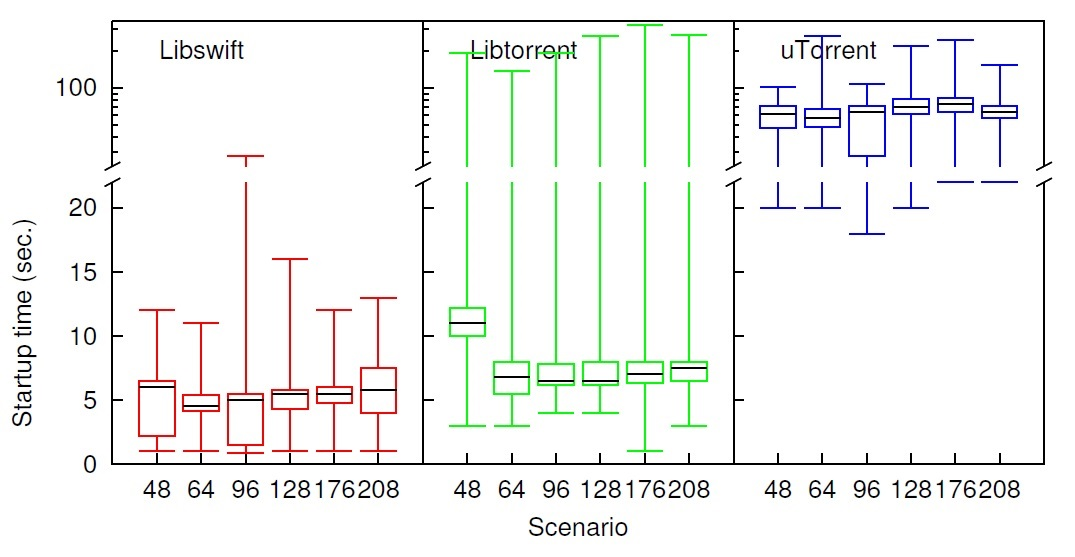
\includegraphics[scale=0.35]{P2P_streaming_protocol/images/start_flashcrowd.jpg}
	\caption{start-up times in a flashcrowd scenario}
	\label{fig:start_flash}
\end{figure}
As can be seen in figure \ref{fig:start_flash} the average start-up time of libtorrent is only a bit higher than with libswift but has a lot of outliers in the high regions, whereas uTorrent has a significantly higher average than the rest.

\begin{figure}[H]
	\centering
	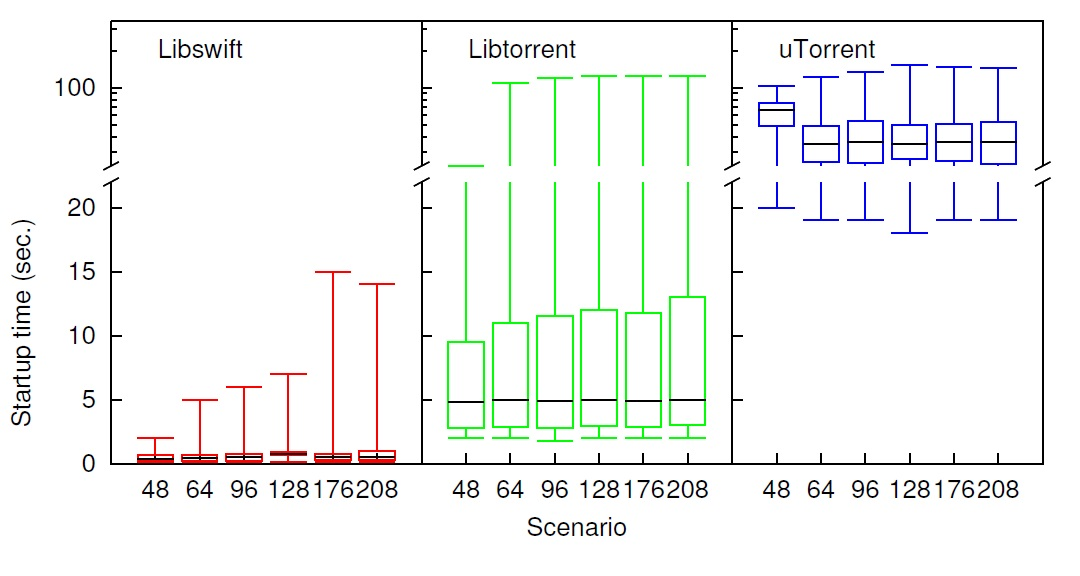
\includegraphics[scale=0.35]{P2P_streaming_protocol/images/start_steady.jpg}
	\caption{start-up times in a steady-state scenario}
	\label{fig:start_steady}
\end{figure}

In a steady-state scenario, Libswift outperforms the other two protocols quite obviously as can be seen in figure \ref{fig:start_steady}.


\subsection{Stalls}

\begin{figure}[H]
	\centering
	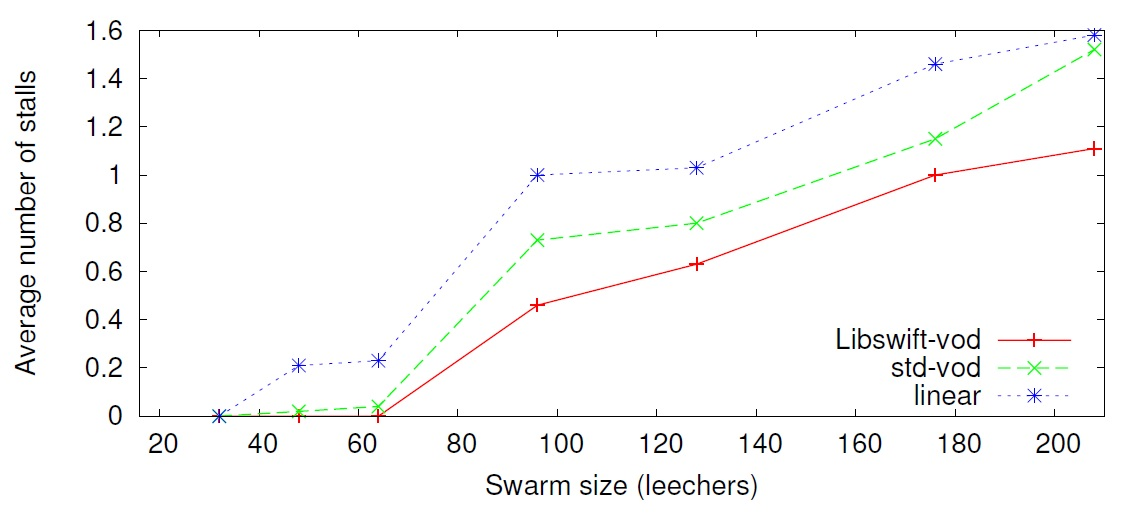
\includegraphics[scale=0.35]{P2P_streaming_protocol/images/stalls.jpg}
	\caption{average number of stalls experienced during playback}
	\label{fig:stalls}
\end{figure}

In figure \ref{fig:stalls} three different download algorithms are compared: 
\begin{itemize}
	\item Linear\\ Only peers further on in the playback are able to provide useful data for newcomers, so there is no global knowledge about data availability in the swarm, making it the worst algorithm in terms of playback stalls.
	\item Standard\\ The standard algorithm holds global knowledge of data availability in the swarm and will download pieces in a rarity-first fashion. It improves on the linear approach as shown in figure \ref{fig:stalls}.
	\item Libswift\\ Libswift has three sets: a low-, medium- and a high-priority set. The high-priority set is the part just after the playback position, and the protocol requests data in-order as these pieces are considered urgent for video playback. The medium- and low-priority set are downloaded in a rarity-first fashion when no pieces from the high-priority set are needed anymore. This can be done because, just like the standard algorithm, Libswift holds global knowledge about data availability. Because the content just after playback position is downloaded first, it scores best on the average number of playback stalls.
\end{itemize}